\def\firstname{firstname}
\def\lastname{lastname}
\def\aufgabenblatt{3}
\documentclass{article}

\usepackage[a4paper, margin=2.5cm]{geometry}
\usepackage{graphicx}
\usepackage[ngerman]{babel} % automatische Silbentrennung
\usepackage[table]{xcolor}
\usepackage{tabularx,array,booktabs,makecell}
\usepackage{titlesec}
\usepackage{amsmath}

\usepackage{fancyhdr}
\pagestyle{fancy} 
\fancyhead[L]{\firstname \: \lastname\\}  
\fancyhead[C]{Bildverarbeitung und Mustererkennung\\Aufgabenblatt \aufgabenblatt}
\fancyhead[R]{\\
\includegraphics[width=0.25\textwidth]{../common/hs_aalen_de.png}}

\fancypagestyle{page1}{
	\fancyhead[L]{\firstname \: \lastname\\}
	\fancyhead[C]{Bildverarbeitung und Mustererkennung\\Aufgabenblatt \aufgabenblatt}
	\fancyhead[R]{ \\
\includegraphics[width=0.25\textwidth]{../common/hs_aalen_de.png}}

}
\setlength{\parindent}{0mm}
\setlength{\parskip}{2.5mm}

\titlespacing*{\section}{0mm}{4pt}{0pt}
\setlength{\headsep}{14mm}

\begin{document}

\thispagestyle{page1} 

\section{Geometrische Operatoren}

Edit the Jupyter Notebook \texttt{Geometric\_Transformation.ipynb}. In this exercise, we will use and understand geometric operations to correct geometric distortions on images.

\subsection{Bilineare Interpolation}

In order to apply geometric operations in a meaningful way, we need the possibility to interpolate. The function \texttt{interpolate\_bilinear} accepts a touple of four rgb colors
($P_{0,0}$, $P_{0,1}$, $P_{1,0}$, and $P_{1,1}$) and a set of coordinates $x,y$. It assumes that the points are located at $0/0$, $0/1$, $1/0$, and $1/1$ respectively and
computes a bilinear interpolated value between them.

\begin{enumerate}

\item[a)] Argue, how this function could be tested.
\item[b)] Setup Unittests for the function.
\item[b)] Implement the function.

\end{enumerate}

I needed the following time to complete the task:

\subsection{Geometric Transformation on Images}

Using the bilinear interpolation, we can now transform images. The function \texttt{transform\_image} accepts an image as numpy array and a geometric transformation $f$, which is also 
a function. Remember, that in Python, functions are just values. In order to compute the new image, which has the same resolution as the original image, \texttt{transform\_image}
transforms each pixel in the output image to the input image. It then performs an interpolated lookup.

\begin{enumerate}

\item[a)] Describe, in your own word, how you are going to deal with pixels outside the input image (you can choose a method).
\item[b)] Describe, how the function could be tested.
\item[b)] Setup Unittests for the function.
\item[b)] Implement \texttt{transform\_image} function.

\end{enumerate}

I needed the following time to complete the task:

\subsection{Affine Transformations}

Now, we will implement a number of geometric transformations. Each of the transformations will be realized by a function that accepts parameters depending on the transformation,
and returns a $3 \times 3$ matrix to realize the operation. 

\begin{enumerate}

\item First, we need a function that applies an affine transformation (multiplication with matrix) to pixel coordinates. This generic function can conveniently be realized using the partial function from functools. The mechanism is demonstrated in the notebook.  
\item Translation accepts two parameters $x$ and $y$ and realizes a translation operation. 
\item Scale accepts two parameters $sx$ and $sy$ and realizes a non-uniform scaling operation.
\item Rotation accepts a single parameter $alpha$ (in radians) and realizes a rotation operation around the coordinate origin. 

\end{enumerate}

For each of the transformations:

\begin{enumerate}
\item[a)] Describe, how the function could be tested. Consider using the inverse operation.
\item[b)] Setup Unittests for the function.
\item[c)] Implement the transformation and its inverse.
\end{enumerate}

Image translated by -50/+22.5 Pixels:

\begin{center}
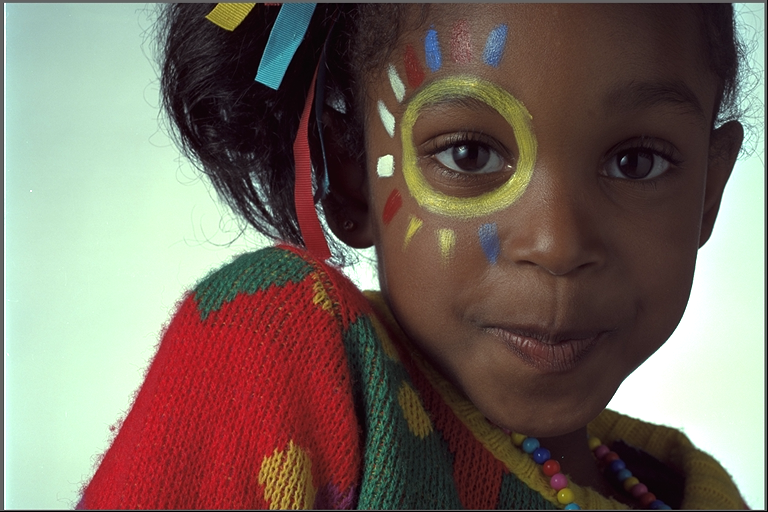
\includegraphics[width=0.45\textwidth]{source\_code/translated.png} \\
\end{center}

Image mirrored vertically:

\begin{center}
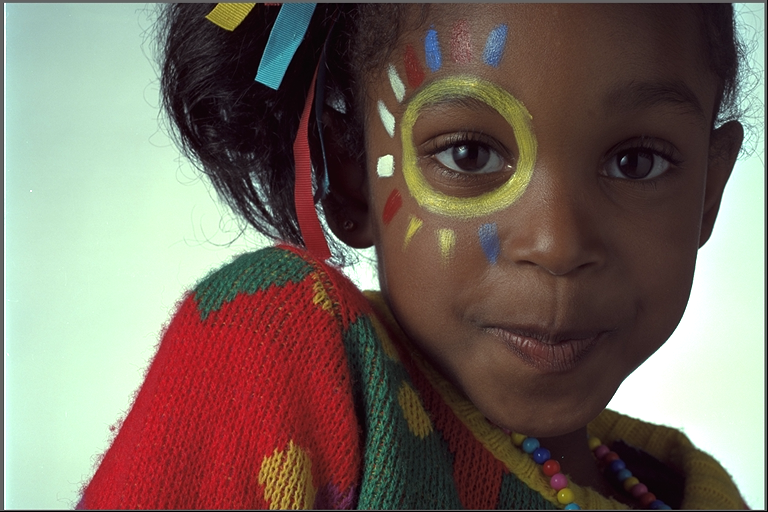
\includegraphics[width=0.45\textwidth]{source\_code/mirrored.png} \\
\end{center}

Image translated by 45 degree around the origin:

\begin{center}
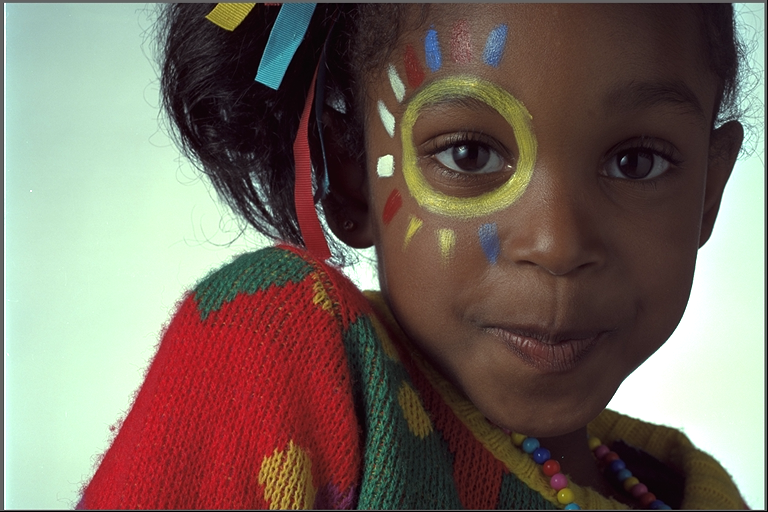
\includegraphics[width=0.45\textwidth]{source\_code/rotated.png} \\
\end{center}

\begin{enumerate}
\item[d)] In order to implement rotations around arbitrary points, we need to concatenate transformations. Implement a rotation functions that accepts three parameters:
$origin\_x$, $origin\_y$ and $alpha$. It rotates by  $alpha$ (in radians) and implements a rotations around the specified origin. Remember how to implement arbitrary rotations: translate the rotation origin to $0/0$, rotate, translate back.
\end{enumerate}

\begin{center}
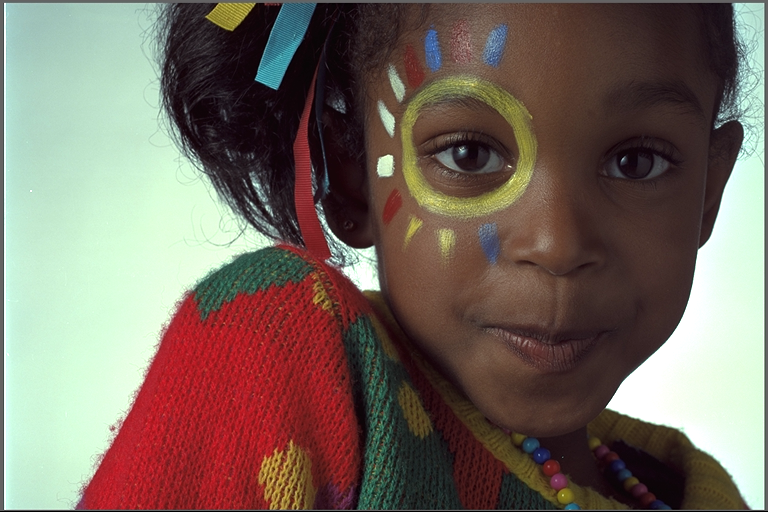
\includegraphics[width=0.45\textwidth]{source\_code/arbitrary_rotated.png}
\end{center}

I needed the following time to complete the task:

\subsection{Perspective Correction}

Now for something a little more fancy. The image \texttt{source\_code/perspective.png} was fotographed from a non-optimal angle. We want to transform it in such a way, that the corners
of the poster become the new corners of the image $(0/0)$, $(0/width)$ and so on. Finding good transformation parameters by trial and error might be time-consuming, though.
In order to solve this problem, we consider the problem as an optimization problem: we use the $argmin$ function to find the suitable transformation matrix, then project the image as required.

The function \texttt{find\_transformation} accepts to sets of four points each ($S=[S_{00},S_{10},S_{01},S_{11}]$ and $D=[D_{00},D_{10},D_{01},D_{11}]$), and returns a $3 \times 3$
transformation matrix $M$ that minimizes the $L_2$ distance between $S$ and $M \cdot D$.

\begin{enumerate}
\item[a)] Describe, how the function could be tested. Consider using the inverse operation.
\item[b)] Setup Unittests for the function.
\item[c)] Implement the transformation and its inverse.
\end{enumerate}

\begin{center}
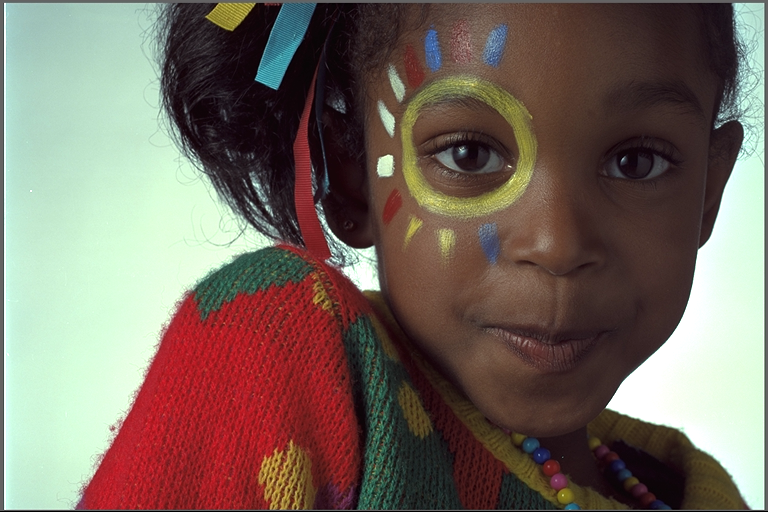
\includegraphics[width=0.45\textwidth]{source\_code/perspective_corrected.png}
\end{center}

\end{document}